\chapter{\label{chap:impl}Implementação}

Para a implementação do simulador, foi escolhida a linguagem C++, por sua grande
flexibilidade e performance, bem como suas poderosas primitivas de controle de
cópia e modificação de objetos.

Os resultados da simulação geram um \textit{log} completo, que é analisado por
uma ferramenta separada, escrita em Python. Esta escolha foi feita pela grande
gama de bibliotecas científicas e estatísticas disponíveis para Python, que
facilitaram enormemente a geração de gráficos para este trabalho.

\section{Cenários}

Aliquam euismod sapien scelerisque hendrerit malesuada. Phasellus rutrum
efficitur quam, sit amet ultricies nunc dignissim a. Sed lorem risus, maximus id
hendrerit non, ultrices at massa.

\section{Simulador}

Proin iaculis purus felis, a ultrices enim convallis in. Integer pharetra
dignissim pellentesque. Nam vitae erat ut risus pellentesque ultricies.

\subsection{Geração de Chegadas}

Vivamus sodales odio malesuada ligula elementum accumsan. Nullam tristique odio
elit, nec dignissim odio tempus sit amet. Aenean semper, purus ac facilisis
tincidunt, sem felis tristique nunc, placerat varius nunc purus vel est. Nullam
convallis turpis efficitur ipsum placerat convallis.

\subsection{Notificação de Eventos}

Donec eu fermentum est. Nunc non nunc gravida, euismod felis sit amet, viverra
turpis. Suspendisse accumsan nisl nec lacinia sollicitudin. Aenean porttitor
efficitur turpis, a malesuada neque mattis in.

\subsection{Atualização do Estado do Sistema}

Mauris ut efficitur justo, et luctus arcu. Vivamus faucibus lorem vel commodo
rutrum.

\section{Estatísticas}

Donec non bibendum sem. Duis tincidunt nisl nulla. Integer congue, risus mattis
vestibulum posuere, metus nisi auctor lacus, sit amet molestie sem mauris sed
lacus. Praesent elementum sapien vitae sapien dictum, ac laoreet purus bibendum.
Nunc sed laoreet turpis.

\section{Geração de Relatórios}

Sed ut faucibus massa. Quisque id ante dolor. Sed et commodo est. Suspendisse
cursus facilisis magna, ac bibendum magna gravida sit amet. Donec sed pretium
enim. Suspendisse dui libero, ornare eu turpis vitae, vulputate cursus diam.

\subsection{Geração de Gráficos}

Os gráficos são gerados com auxílio da biblioteca Seaborn~\cite{seaborn}, em Python.
Esta biblioteca possui primitivas poderosas de cálucos estatísticos e geração de
gráficos, garantido a corretude da análise dos resultados com um esforço reduzido.

Pode-se ver na Figura~\ref{fig:seaborn} um exemplo da expressividade desta ferramenta.

\begin{figure}[htb]
  \centering
    \begin{minted}[
frame=lines,
framesep=2mm,
baselinestretch=1.2,
linenos
]{python}
    def averageTravelTime(data):
        data['travelTime'] = data['dropoffTime'] - data['pickupTime']
        g = sns.FacetGrid(data, col='dropoffFloor', row='arrivalFloor')
        g = g.map(sns.barplot, "travelTime", orient='v')
    \end{minted}
  \caption{Código em Python para gerar o gráfico da matriz de tempo de espera.}
  \label{fig:seaborn}
\end{figure}

Na segunda linha da Figura~\ref{fig:seaborn}, utiliza-se a ferramenta de
vetorização para calcular-se a diferença entre o tempo de entrega do passageiro
(\textsf{dropoffTime}) e o tempo em que ele foi pego pelo elevador
(\textsf{pickupTime}). Note que nem mesmo um \textit{loop} é necessário. A
biblioteca infere isto e calcula para todos os valores.

Nas linhas seguintes, apenas diz-se o que se quer nas colunas e linhas do
gráfico, e o que deve ser representado pelas barras verticais.

Um exemplo de gráfico gerado por este código está na Figura~\ref{fig:seaborn:exemplo}.

\begin{figure}[htb]
  \centering
  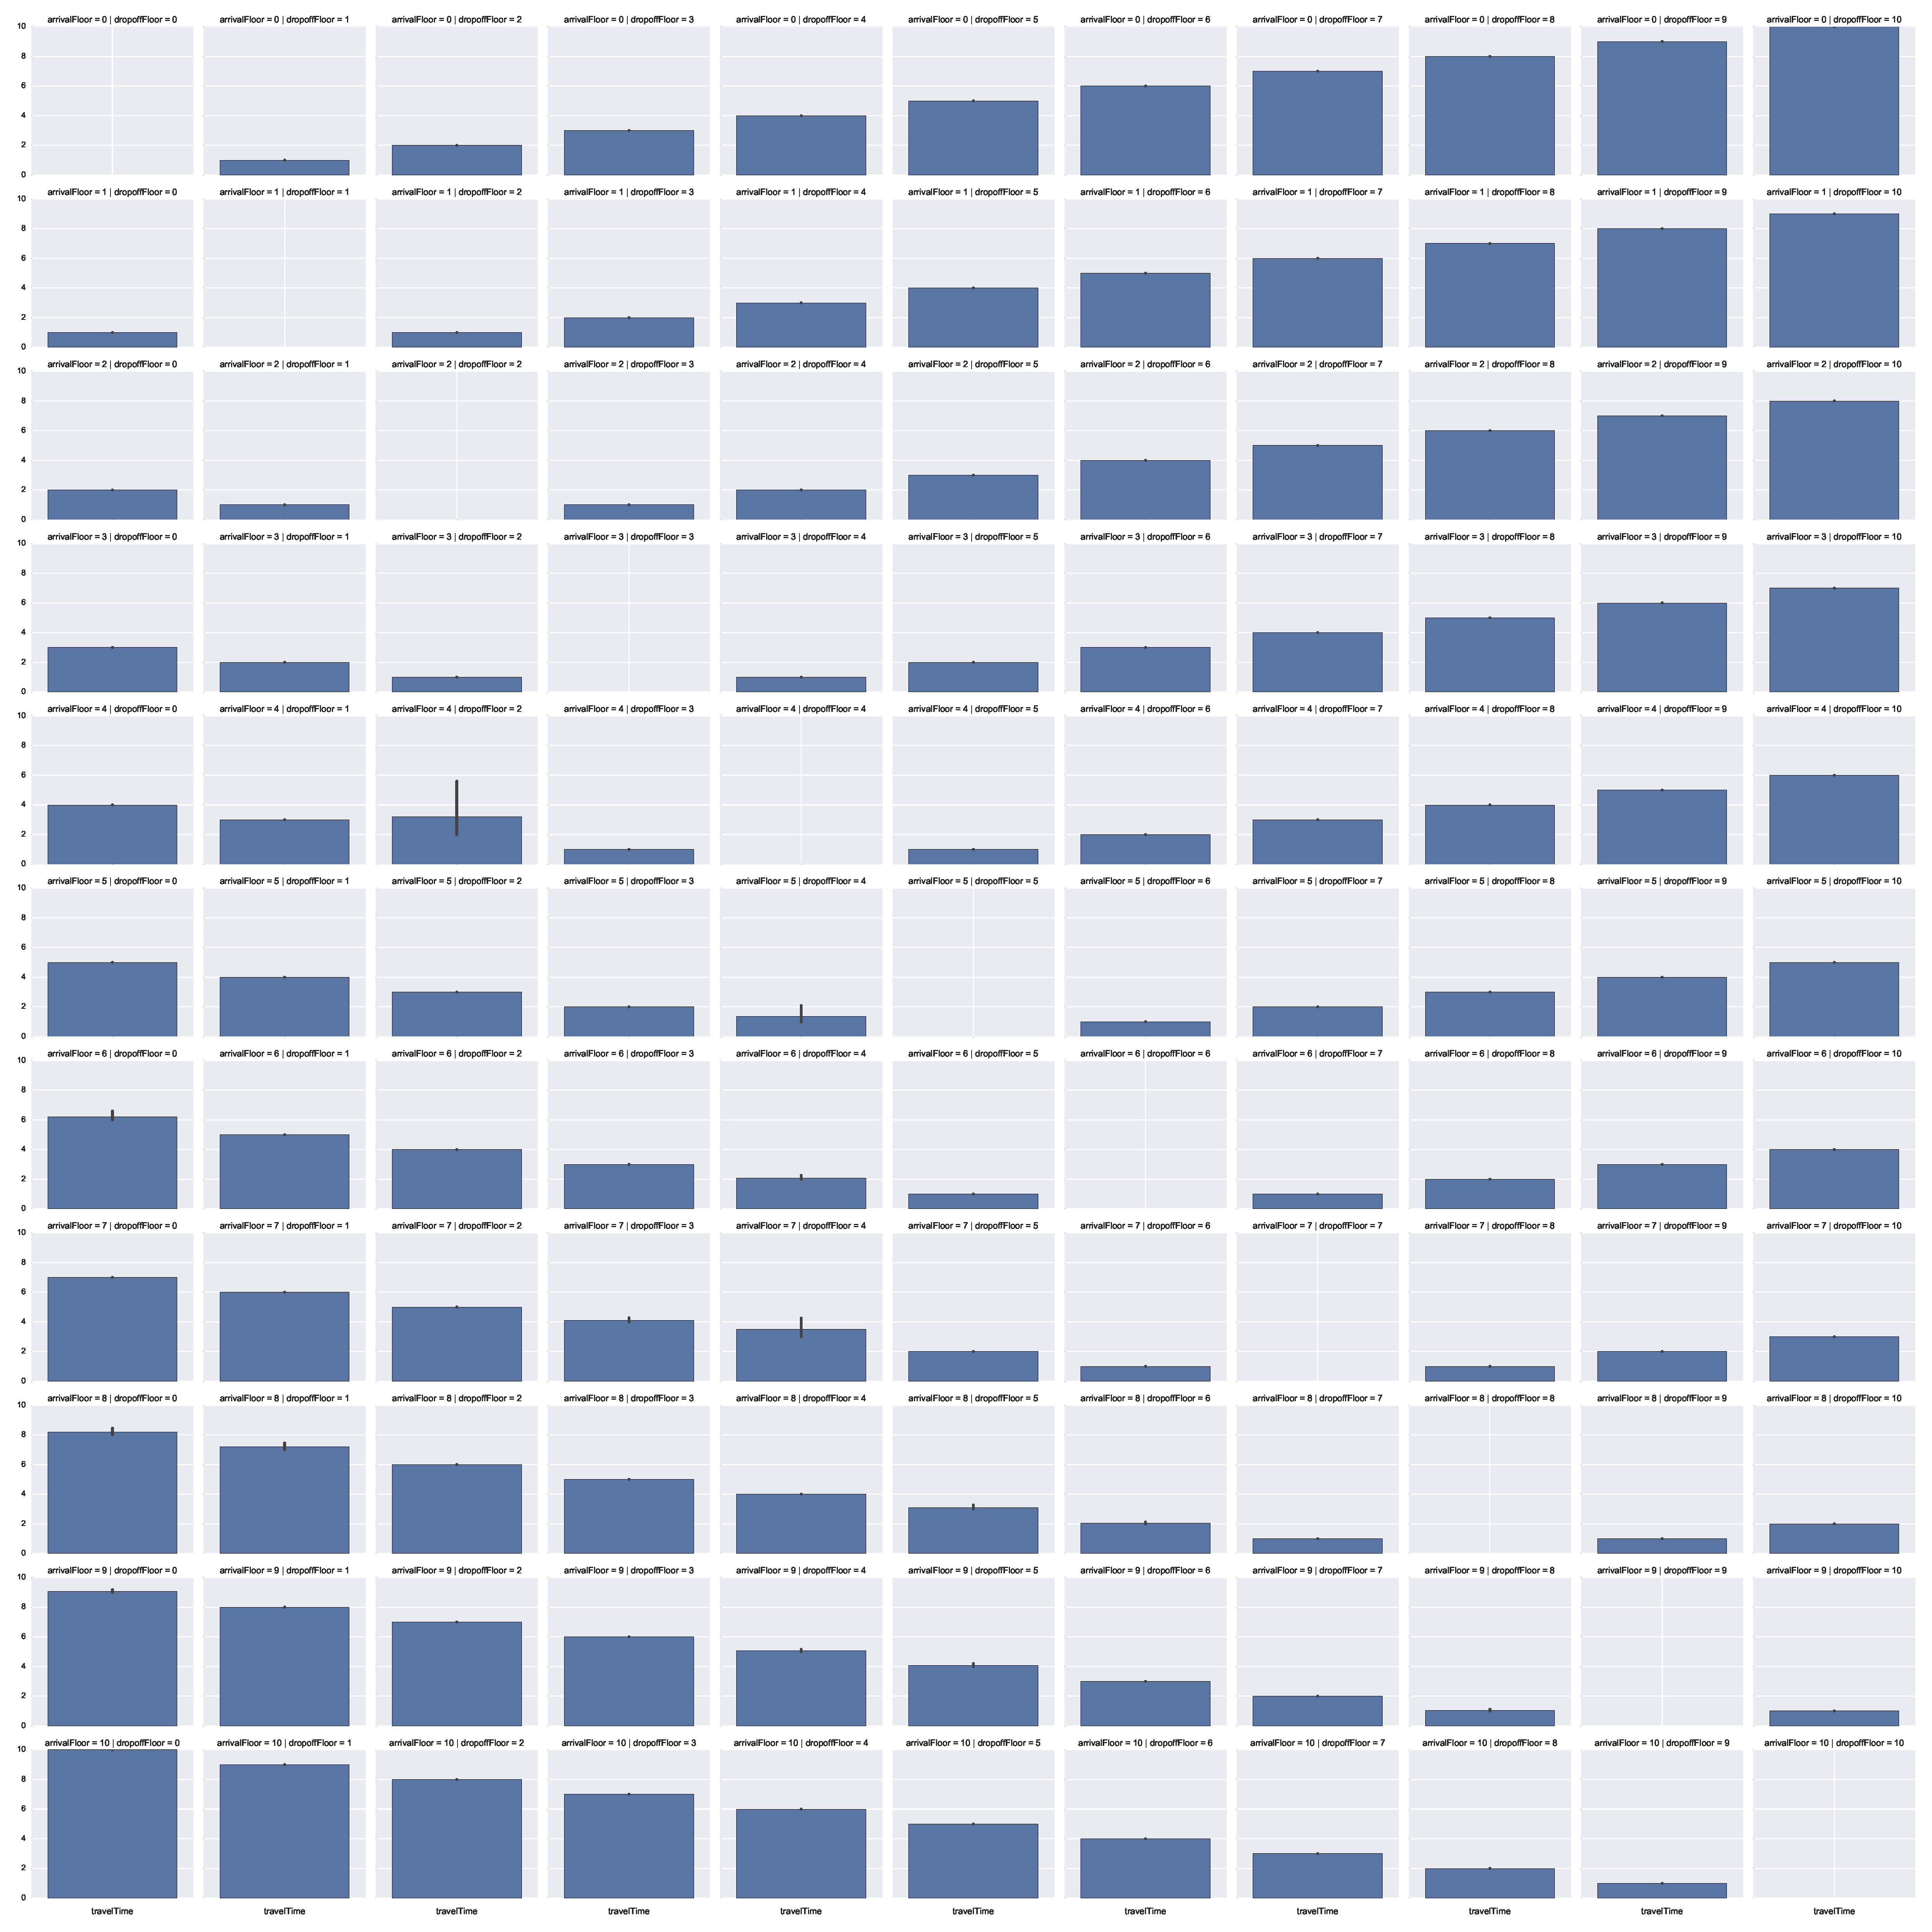
\includegraphics[scale=0.1]{img/seaborn_example.eps}
  \caption{Um exemplo de gráfico gerado pelo código da
    Figura~\ref{fig:seaborn}.}
  \label{fig:seaborn:exemplo}
\end{figure}

\section{Schedulers}

Maecenas facilisis velit et mollis rhoncus. Nam iaculis lacus non lorem aliquet
sollicitudin. In ligula ex, rhoncus nec lacinia et, vehicula ac ligula.

\subsection{Classe Base}

Vestibulum ante ipsum primis in faucibus orci luctus et ultrices posuere cubilia
Curae; Ut sed diam sed libero dignissim viverra in ut ante.

\subsection{Simple}

Sed ac odio placerat, mattis lectus non, consequat metus. Nam vitae urna
pulvinar, lacinia mi ut, maximus nulla.

\subsection{Planning}

Aliquam erat volutpat. Curabitur quis velit libero.
Sed et erat urna. Curabitur ullamcorper, sapien quis facilisis luctus, neque
dolor volutpat neque, a lacinia libero tellus at est.

\section{Funções de Custo}

Vivamus interdum nunc ligula, et consequat tortor fermentum at. Aenean turpis
ante, tempor quis dictum sit amet, ullamcorper et justo.

\subsection{Classe Base}

Suspendisse porta, eros non faucibus eleifend, nunc arcu tempor mi, ut rutrum
orci augue id ligula. Quisque ac augue sed metus mollis tempus. Duis a tincidunt
justo.

\subsection{Dummy}

Proin tincidunt elementum nisi, vel ultrices neque porttitor id. Vivamus vitae
libero velit. Nullam mollis a enim sit amet eleifend. Donec id congue ex.

\subsection{Random}

Sed vehicula justo nec euismod maximus.

\subsection{Nearest Neighbour}

Aenean odio metus, molestie at ligula nec, dignissim blandit ante. Curabitur
consectetur tortor ac lectus egestas tempor.

\subsection{Nearest Neighbour Melhorado}

Curabitur condimentum in mi in euismod. Curabitur rhoncus euismod sapien eu elementum. Curabitur quis odio in nunc vulputate placerat. Fusce tristique placerat massa, eu sollicitudin libero elementum et.

\subsection{Weighted}

Vestibulum ante ipsum primis in faucibus orci luctus et ultrices posuere cubilia Curae; Sed congue quam sapien, ac fermentum libero vulputate vitae.